\documentclass[../report.tex]{subfiles}
\begin{document}
\graphicspath{{img/}{../img/}}
\section{Context awareness}
To be able to make a context-aware framework, we first had to investigate what context and context-awareness is in a computer science perspective.

Context-awareness is a term associated with Ubiquitous computing. Ubiquitous computing, ubicomp, was coined in the early nineties by Mark Weiser whose vision was to make technology that could seamlessly assist in everyday tasks. Weisers research-unit at Xerox PARC developed some of the first mobile devices, and the development of ubi computing clearly reflects in todays technology boom of smart phones and tablets.

For a system to seamlessly interact with a human the system must acquire knowledge to the current situation or \textit{context}. Many of the publications on the subject describes context different, but the one description fitting best our understanding was coined by Dey and Abowd whom described context as:

\blockquote{\textit{Any information that can be used to characterize the situation of an entity. An entity is a person, place or object that is considered relevant to the interaction between a user and an application, including the user and application themselves.}} \cite{Dey and Abowd (2000)} 

When humans interact, they can interpret the ongoing situation from implicitly understanding body language, tone of voice, the surrounding environment as well as maybe having a relation to the person or knowing about past and future events. These \textit{context informations} is essential factors in effective communication. By increasing the amount of context information available to computers, human-machine interaction can be improved.\\

% Holy grail is to understand and perform human intent
\todo{We strive to understand human intent, with sensors. We might not catch it all, but that's not because it's a machine, this can happen in all kinds of interactions; culture differences... Something on this}


Much research have been done in increasing the available amount of context-information, but also heightening the quality and correctness of the information is in focus. As the amount of context increases, the context-aware application becomes able to take actions without explicit user input. When doing so, action can be taken on wrong or typically incomplete snaps of context. 


\blockquote{\textit{Intelligibility and control are important user concerns in context-aware applications. They allow a user to understand why an application is behaving a certain way, and to change its behaviour.}} \cite{Dey and Newberger (2009)}
\todo Write more about context accuracy


\section{Context aware frameworks}
% Frameworks have been developed to accomadate this
To support application developers a number of context-frameworks have been developed. When looking at the frameworks mainly two approaches were used: Blackboard and Widget-based architecture.

The blackboard approach is a centralized solution. Sensors and application are connected to the blackboard and when ever a new sensor state is available a post-it, an entry to the database, is put on the blackboard. The application can at will look through the blackboard and search for context it might find relevant. The blackboard abstracts away the sensor allowing the client to focus on only the context information. 

\begin{figure}
\centering
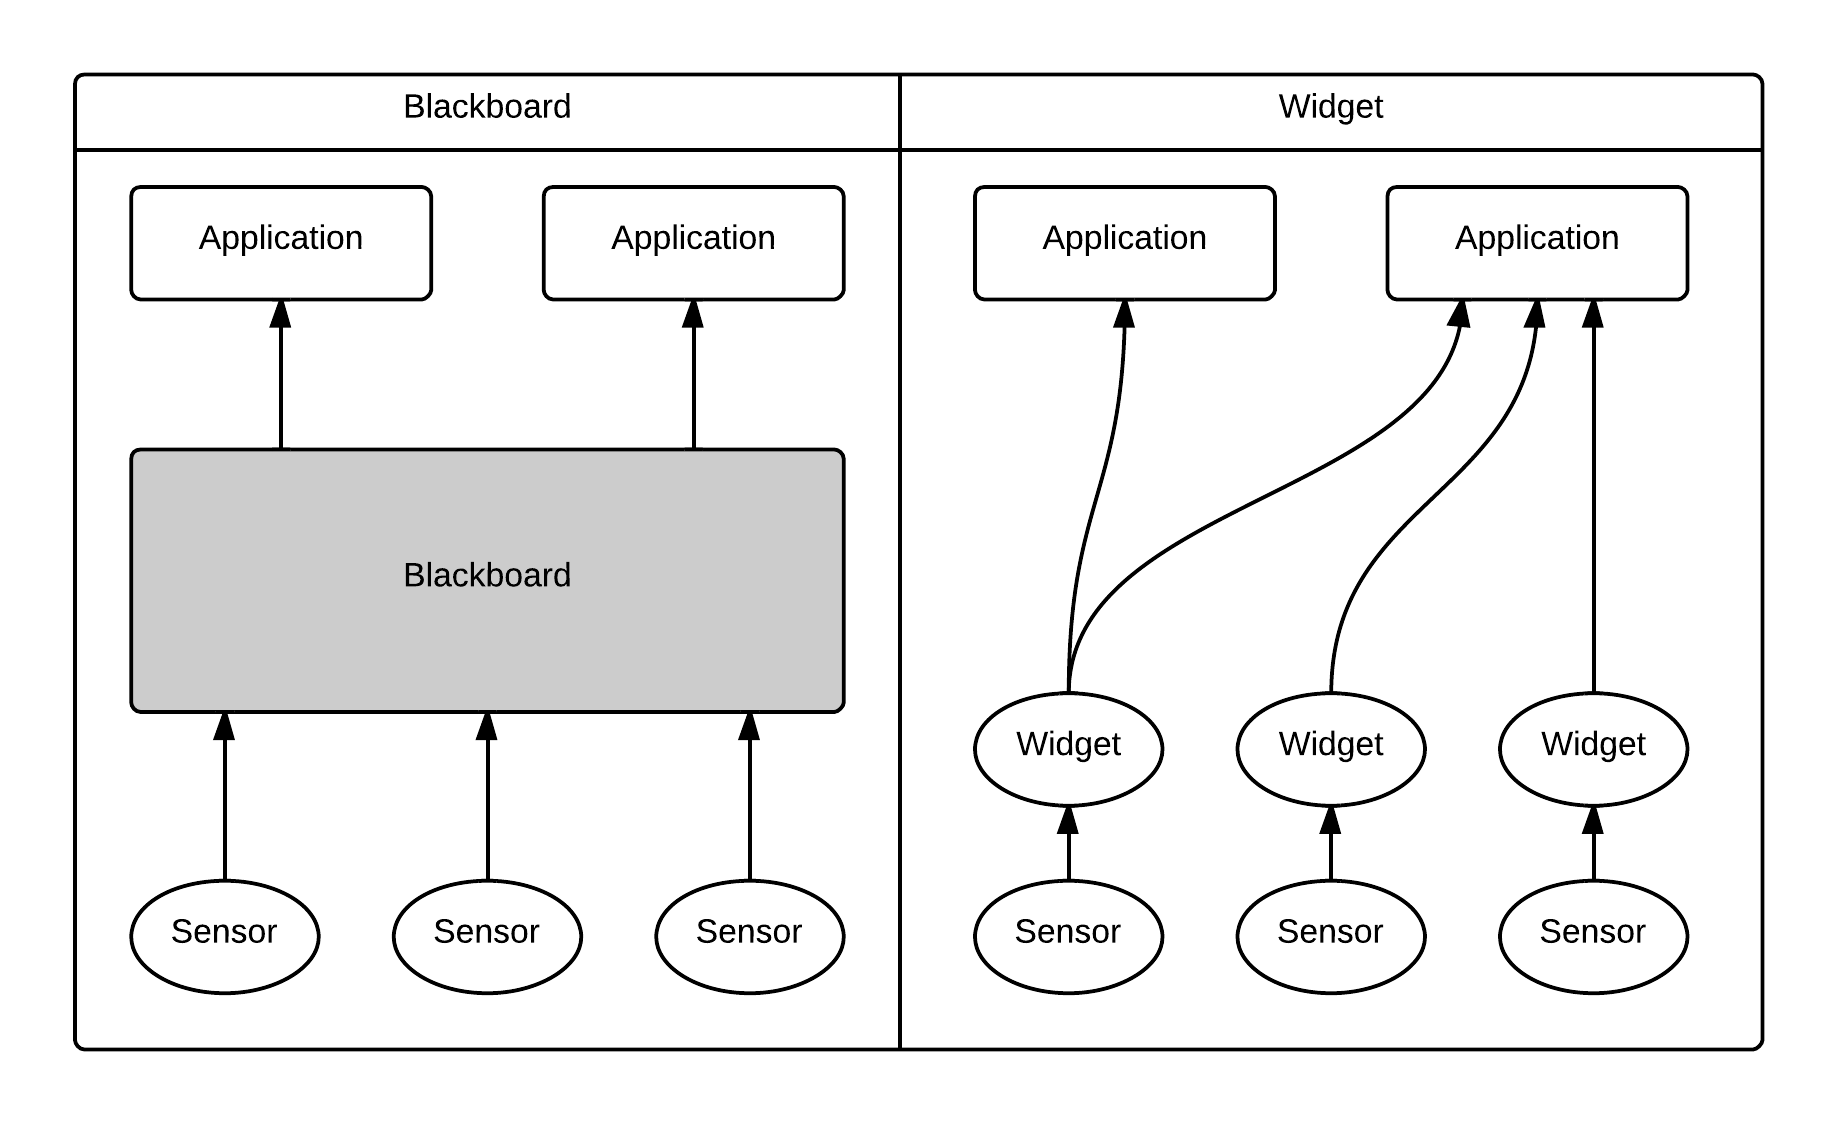
\includegraphics[width=\linewidth]{blackboard-widget.png}
\caption{Blackboard and widget-based approach}
\label{fig:blackboard-widget}
\end{figure}

The widget approach is an object-oriented distributed solution. Sensors encapsulated by widgets are available for application subscription. The solution is event based and applications are notified whenever a change to the sensor is occurring. This solution is object-oriented as the context is modelled with objects sent from sensor to application. This time and spare coupled solution stands in contrast to the blackboard approach which is a database and is therefore time- and space uncoupled.

The solution differs a lot in the way the model context, but the main differers is in the way of delivering context from sensor to application. The solutions stands in great contrast when looking at space and time coupling. To briefly describe the theory, space coupling is weather or not the sender knows who the receiver of a message is. Time coupling is if the given message is only available in real-time. 

Where the blackboard at any time offers applications to go though it's context database, it does not offer notifying the application, as the blackboard is space uncoupled, and does not know about the application. The widget solution offers live updated only when they happens and only to the applications subscribing for the update.

Both solutions are very useful in different applications.

\todo Should the two examples stay?\\
For example a hospital system where you want to use the context framework to track patients, the blackboard solution seams to meet requirements best as you can, when needed, look up a patients whereabouts in the hospital.

For a home automation system using sensors, sensor input is only interesting the moment it happens, and only to actuator whom it concern. When a person enters the room the light should go on instantly, only in the room where the person entered and only at the given time. 


\end{document}